\documentclass{memoir}

\usepackage{import}
\import{../}{gov-style}
\addbibresource{../thesis.bib}

\begin{document}
\section{A grand theory of intelligence}
\subsection{The takeaways}

For someone my age, born in the 1990s, it is difficult to remember remember a time before Google Earth, the PATRIOT act, and Guantanamo. The omnipresence of photographic satellites feels unnervingly benign today---in the same way that having immense amounts of personal data collected without our knowledge feels regrettable but inevitable, your tithe for living in the \nth{21} century. Why \emph{shouldn't} adversarial states attempt to collect as much information as they can, using the whatever means at their disposal? They are, after all, just observing. Downloading government records feels like fair game; it feels like something a spy would do by inserting a thumb drive into a computer; it feels like espionage.

But the reason spy satellites, data breaches, and wiretaps feel like espionage is because we treat them that way, not because something about them is obviously acceptable. Chapters 3 and 4 make clear that the association of certain activities with espionage is a deliberate choice, and a choice that must be renewed with each new technological means. The SR-71 Blackbird, a more recent reconnaissance aircraft, did not require a whole new set of norms when it was introduced; the U-2 had already blazed a trail for the role of a spy plane in international affairs. The internet, by contrast, was a radical new domain for international competition. Like outer space and the open skies, espionage through the internet did not necessarily start as fair game---it became such because policymakers deliberately responded to data breaches the way they would have responded to espionage. The choice to respond that way is ongoing, and any actor could defect at any time.

% What we have is a carefully preserved system

% As the rest of the conclusion presents a very optimistic take on intelligence generally, it is important to acknowledge that the scandals surrounding national intelligence agencies are well-documented, and in no way do I seek to excuse them. This thesis does not even touch the murky world of covert action that is most often associated with the CIA, including the attempted assassination of Fidel Castro, the Guatemalan \emph{coup d'\'etat}, and the Iran Contra affair. These are not uniquely American sins either. Though a lot of information about the inner workings of the KGB and the GRU is lost to history, modern Russian intelligence was implicated in an assassination attempt as recently as 2018. Illicit covert actions are disturbing elements of the intelligence apparatus which, morally, cannot be entirely separated from the pure information-gathering efforts that I have examined. Nonetheless, this thesis focuses on an element of American and Soviet intelligence that I believe to be a strong net positive for international security---the norm that states have a tacit right to verify intelligence through espionage, and that espionage countermeasures will be limited to certain narrow measures.

My goal with this thesis is to situate peacetime espionage within the existing literature on international security, and apply the lessons from that analysis to the evolving practice of cyber-espionage. The intersection of espionage and international relations has been studied before---beginning, in the modern context, as far back as 1962---but the role of espionage in deescalating conflict is typically relegated to historical accounts of individual moments where Great People properly interpreted---or fatally misunderstood---the information that their intelligence operations provided them. In choosing to focus on decisions made by Eisenhower and Khrushchev, I am partially guilty of that as well, but I try to highlight the way in which both of those leaders set precedents designed to outlast them. By analyzing the application of espionage norms to a variety of technologies, instead of just the individual decisions that were made using them, I can start the conversation about how these norms operate to deescalate conflict independent of the leaders that promote them.

The strategic choices that ultimately normalized the use of spy planes and spy satellites are choices that can be and have been repeated. When the United States first introduced these novel spy technologies to the world, it made a deliberate effort to associate them with the espionage tradition. It appears that cyber-espionage has been given that same association---hence the name---but because it is happening contemporaneously, we, the public, do not have the same ability to trace the process. Certainly there are obvious signs that some types of cyberattacks are considered espionage---when congresspeople literally say so---but we deserve to know how that distinction gets made, what policies govern the diplomatic response, and whether those policies benefit the interests of the United States. In the following sections, I will note how the United States built that connection historically, and connect it to the ongoing choices that the United States makes to promote espionage norms in cyberspace today.

Intelligence serves a crucial de-escalatory purpose in the international system, but espionage norms are not magic, and the careful technological \emph{d\'etente} that years of space peace and Open Skies have accustomed us to should not taken for granted. The equilibrium is constantly under siege from rogue actors, revisionist powers, and even domestic political factions that push policymakers respond more aggressively to cyber-espionage. The United States greatly benefits from a world in which global communication systems are considered off-limits to attack, and ought to be working actively to preserve it. The space age is a phenomenal example of how that can be achieved. Intelligence norms worked in the 1960s to marry security concerns---verifying arms control agreements---with the best interests of the entire world---that space be preserved as an arena where countries compete to out-innovate, rather than out-weaponize. A similar outcome is possible with the internet today, but it will not happen automatically. In the final section, I will talk about some of the greatest threats to peaceful intelligence gathering today, and how the United States might preserve a ``peaceful uses of cyberspace'' policy from which, like the ``peaceful uses of outer space,'' it stands more to gain than any other.

\subsection{Espionage in the nuclear age}
My theory concludes that the diplomatic equilibrium preserving espionage exists because virtually all states believe that a world with more intelligence is one that is less likely to lead to miscalculation, even if that intelligence sometimes comes at a personal cost. That miscalculation could be minor---an arms build-up that eventually halts, as seen with the development of ASAT weapons---or it could that final miscalculation that has haunted IR since the advent of ballistic missiles---the specter of total nuclear war. Glaser acknowledges the highly risk-averse nature of the Cold War, and I believe that the evidence presented in this thesis consistently demonstrates a bias on the part of all policymakers towards a world in which all actors are making the most informed decisions possible, because it is in the best interest of all actors not to annihilate all life on Earth.

It should go without saying that intelligence is not always used to reduce security tensions---it can just as easily have a net neutral, or even net negative effect. The most transformative intelligence failure of my lifetime was the 2003 invasion of Iraq, now considered, by virtually all ends of the political spectrum, to have been a colossal mistake. Much of the blame for that mistake rests at the feet of the American intelligence community, which the bipartisan Robb-Silberman Commission determined ``was dead wrong in almost all of its pre-war judgments about Iraq's weapons of mass destruction.''\footcite{commission_on_the_intelligence_capabilities_of_the_united_states_regarding_wmds_final_2005} The technological, organizational, or political changes that could have led the intelligence community to a different conclusion are a subject for a different thesis (or theses), but I invoke the Second Gulf War as a reminder that more trust in intelligence does not always lead to more secure outcomes, and my conclusion should not be interpreted as such.

I do believe, however, that preserving espionage as an intelligence-gathering practice leads to more secure outcomes in the international system. Espionage gives security-seeking states a means to verify the intent and capabilities of their adversary without fundamentally altering that relationship. When both parties stay with the accepted bounds, they successfully cooperate to keep their intelligence clashes quarantined. The next section will address exactly how those bounds are ported to new technologies.

% The second chapter established that the legal gray area which espionage occupies gives states the ability to denounce espionage against them without committing to legal regime that would them accountable for doing the same. A spy who is caught will likely be punished in the harshest possible by domestic courts, but rarely will the state that ran them feel any significant consequences beyond the loss of their agent, and at worst, some embassy personnel. Spying is therefore not condoned exactly, but states can be reasonably confident that their attempts to spy on another state will not jeopardize other elements of that relationship. The state might get caught, embarrassed, and have elements of their intelligence operations curtailed, but as the operation consists entirely of observation, then in all other respects the state will remain diplomatically unscathed.

Chapters 3 and 4, which examined aerial and satellite reconnaissance, would at first glance appear to be limit-testing cases, because they introduced brand new technologies into the world of espionage. In fact, they are just the opposite. Eisenhower was not interested in pushing the limits; he wanted his new technologies to definitively fit within the bounds of what the Soviet Union would consider espionage. Even though the world had never before seen a reconnaissance satellite, Eisenhower wanted it to feel like a spy. He wanted to make it clear that his new devices intended to play by the rules of the game.

\subsection{New dogs, old tricks}

% The capabilities are no longer symmetrical in the easy way that dueling embassy operations are.

Linking the spy plane to intelligence norms worked because the United States fully committed to building the project around that requirement. Like a human spy, the spy plane and the spy satellite were purpose-built to be information gatherers. It would have been impossible to mistake them for anything else. Neither the spy plane nor the spy satellite had weapons of any kind, and their operation was controlled by civilian intelligence agencies. Like Tolkachev, they covertly observed about Soviet military developments.

Because the spy plane was, in story as well as fact, a civilian intelligence operation, it was still considered within the rules of the game after the plan went wrong. U-2 pilots were given a suicide capsule, but  that was mostly for their psychological benefit, because, in a macabre twist, the pilots weren't supposed to survive a crash at all. The United States originally went with the weather craft story because Eisenhower had been assured that Gary Powers could not possibly have survived.\footcite[p.~35]{lindgren_trust_2000} When Powers confessed to his Soviet captors, he told them, truthfully, that he was a civilian pilot with the CIA. His cover had been blown, but underneath it he was still a spy, and in pretty much all respects he and the U-2 were treated accordingly.

The evidence of the empirical chapters makes a strong case that framing the U-2 and Corona projects as intelligence efforts---in everything from their design to the bureaucracy that administered them---effectively reduced the diplomatic consequences when that technology was discovered, but it should be noted that the evidence is circumstantial. We know that Eisenhower thought it important that the CIA run the U-2 program instead of the Air Force, and we know that the USSR did not bomb the base from which the U-2 was launched, in retaliation for the deeply illegal overflight. It is tough to say that one caused the other. We know that the USSR traded Gary Powers for a spy, and the Khrushchev deceitfully downplayed the frequency of reconnaissance overflights in his memoirs. Khrushchev's attitude towards the incident is very similar to how states routinely minimize the frequency and effect of espionage against them, but without a quote saying as much, it would impossible to assign him that exact motive.

Whatever other circumstances might have influenced the Soviet response to American technical reconnaissance, we know for certain that Eisenhower sought to make build a clear association between between technological reconnaissance instruments and human spies, and that he was successful. The U-2 essentially invented the term ``spy plane,'' and appeared as such in \emph{The New York Times}. In the early days of the Corona project, the Soviets press decried the American attempt at ``espionage from space.'' Even if a norm against ASATs had not followed, the United States had already succeeded in associating their new technology with a set of norms that limited how much it could be punished. This association is not an exact science; The rules of the game are entirely comprised of tradition and familiarity, and when you replace a human with a manned aircraft, or a manned aircraft with a beeping ball of metal, it looks less like something that intelligence professionals are used to responding to.

Eisenhower maximized the odds that the Soviet Union would see spy planes and spy satellites as espionage equipment, but the margin of his success was slim. One does not know what would have happened diplomatically had it turned out that the U-2 was also capable of dropping a bomb, but we do know that American and Soviet restraint on weaponized satellites was decisive in preserving the freedom of space. Deploying an orbital bomb or an ASAT would have completely changed the space race. Both sides were able to agree with spy satellites did not constitute a provocation, but had either side deployed a space weapon that clearly did, then there is no guarantee that spy satellites would have been immune from the backlash. Preserving the norms of espionage in space required that space not be used for weapons.

\subsection{Returning to explanations}
% One of the central puzzles of the previous two chapters is how to explain why the Soviet Union did not respond more aggressively to American technological espionage, even as it eviscerated key elements of the Soviet security position. The U-2 flew 4 years worth of missions before the USSR shot one down, and the fleet of spy satellites that orbit the Earth remain untouched to this day. The United States had no established right to use either of those tools, but as it continued to do so, the Soviet means of discouraging spy planes and spy satellites proved consistently ineffective. Meanwhile, American photo-reconnaissance vastly improved NATO missile targeting and revealed that Soviet retaliatory capabilities were far behind what Khrushchev had claimed. Starting in the late 1950s, the Soviet Union understood, without questions, that photo-reconnaissance was leading to major relative gains for the United States.


\section{Satellites}
% The psychological bias that intelligence is less threatening than traditional military operations still existed, but it had to be deliberately associated with the new technological capabilities---and it had to supersede existing norms from other fields of IR.

% Conclude with LBJ and final acknowledgment

\section{Satellites from Kennedy to today}
Today, space has been thoroughly militarized, but not weaponized. The difference between the two is significant; weaponization requires the placement of space-based devices that have destructive capacity, such as an orbital satellite loaded with nuclear bombs, while militarization is simply the use of space-based devices to facilitate military operations.\footcite[p.~3]{mowthorpe_militarization_2004} Currently no one faces the threat of an attack originating from space, but an incredible number of more traditional American military capabilities rely on the network of satellites. According to the official government website, The Global Positioning System (GPS) alone is used by the DoD for precision guided munition strikes, force tracking, search and rescue, and remote piloting of unmanned aerial vehicles.\footcite{national_coordination_office_for_space-based_positioning_navigation_and_timing_federal_2018} A fleet of spy satellites, built and maintained by the National Reconnaissance Office since 1961, take high-resolution photos of places Gary Powers could never have reached.\footcite{national_reconnaissance_office_about_2019} The many commercial and civil satellites operated by American entities have military applications as well.

\subsection{Satellites today}
There are a lot of possible targets.\footcite[A few satellites are listed as dual-purpose (i.e. Government/Military), and those are counted twice, once for each purpose. For instance, the data shows that the US is currently operating 830 satellites, while adding up the bars in this chart would give you 966. I made this choice to emphasize the dependency of various social systems on the existing satellite infrastructure.]{union_of_concerned_scientists_ucs_2018}


\begin{figure}[ht]
  \centering
  % Created by tikzDevice version 0.12 on 2019-05-03 23:25:55
% !TEX encoding = UTF-8 Unicode
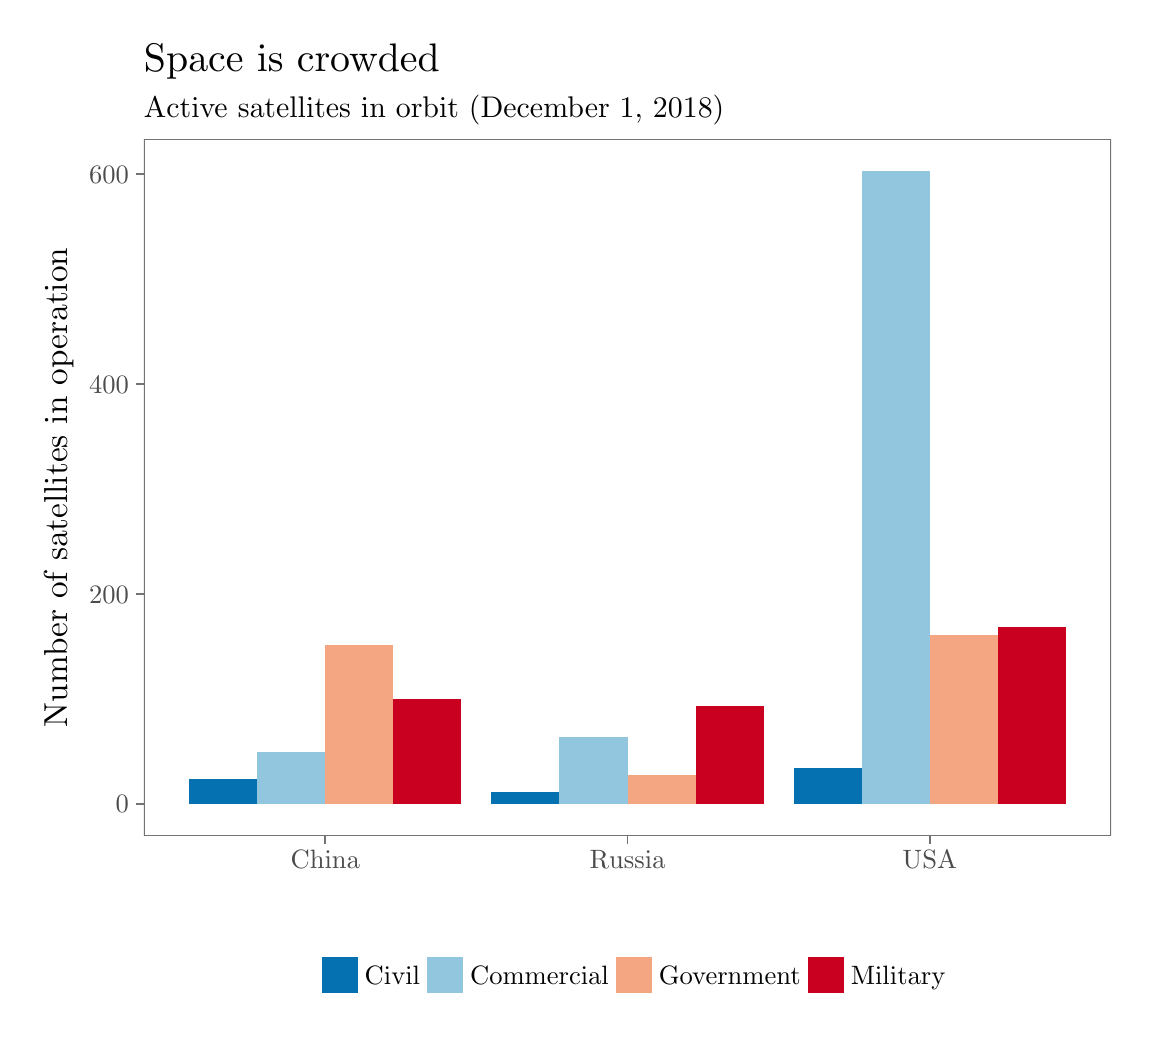
\begin{tikzpicture}[x=1pt,y=1pt]
\definecolor{fillColor}{RGB}{255,255,255}
\path[use as bounding box,fill=fillColor,fill opacity=0.00] (0,0) rectangle (397.48,361.35);
\begin{scope}
\path[clip] (  0.00,  0.00) rectangle (397.48,361.35);
\definecolor{drawColor}{RGB}{255,255,255}
\definecolor{fillColor}{RGB}{255,255,255}

\path[draw=drawColor,line width= 0.6pt,line join=round,line cap=round,fill=fillColor] (  0.00,  0.00) rectangle (397.48,361.35);
\end{scope}
\begin{scope}
\path[clip] ( 42.01, 69.49) rectangle (391.48,320.95);
\definecolor{fillColor}{RGB}{255,255,255}

\path[fill=fillColor] ( 42.01, 69.49) rectangle (391.48,320.95);
\definecolor{fillColor}{RGB}{202,0,32}

\path[fill=fillColor] (132.11, 80.92) rectangle (156.68,118.83);
\definecolor{fillColor}{RGB}{244,165,130}

\path[fill=fillColor] (107.53, 80.92) rectangle (132.11,138.17);
\definecolor{fillColor}{RGB}{146,197,222}

\path[fill=fillColor] ( 82.96, 80.92) rectangle (107.53, 99.50);
\definecolor{fillColor}{RGB}{5,113,176}

\path[fill=fillColor] ( 58.39, 80.92) rectangle ( 82.96, 90.02);
\definecolor{fillColor}{RGB}{202,0,32}

\path[fill=fillColor] (241.32, 80.92) rectangle (265.89,116.18);
\definecolor{fillColor}{RGB}{244,165,130}

\path[fill=fillColor] (216.75, 80.92) rectangle (241.32, 91.16);
\definecolor{fillColor}{RGB}{146,197,222}

\path[fill=fillColor] (192.17, 80.92) rectangle (216.75,105.19);
\definecolor{fillColor}{RGB}{5,113,176}

\path[fill=fillColor] (167.60, 80.92) rectangle (192.17, 85.09);
\definecolor{fillColor}{RGB}{202,0,32}

\path[fill=fillColor] (350.53, 80.92) rectangle (375.10,144.61);
\definecolor{fillColor}{RGB}{244,165,130}

\path[fill=fillColor] (325.96, 80.92) rectangle (350.53,141.96);
\definecolor{fillColor}{RGB}{146,197,222}

\path[fill=fillColor] (301.38, 80.92) rectangle (325.96,309.52);
\definecolor{fillColor}{RGB}{5,113,176}

\path[fill=fillColor] (276.81, 80.92) rectangle (301.38, 93.81);
\definecolor{drawColor}{gray}{0.45}

\path[draw=drawColor,line width= 0.6pt,line join=round,line cap=round] ( 42.01, 69.49) rectangle (391.48,320.95);
\end{scope}
\begin{scope}
\path[clip] (  0.00,  0.00) rectangle (397.48,361.35);
\definecolor{drawColor}{gray}{0.30}

\node[text=drawColor,anchor=base east,inner sep=0pt, outer sep=0pt, scale=  0.96] at ( 36.61, 77.62) {0};

\node[text=drawColor,anchor=base east,inner sep=0pt, outer sep=0pt, scale=  0.96] at ( 36.61,153.44) {200};

\node[text=drawColor,anchor=base east,inner sep=0pt, outer sep=0pt, scale=  0.96] at ( 36.61,229.26) {400};

\node[text=drawColor,anchor=base east,inner sep=0pt, outer sep=0pt, scale=  0.96] at ( 36.61,305.08) {600};
\end{scope}
\begin{scope}
\path[clip] (  0.00,  0.00) rectangle (397.48,361.35);
\definecolor{drawColor}{gray}{0.45}

\path[draw=drawColor,line width= 0.6pt,line join=round] ( 39.01, 80.92) --
	( 42.01, 80.92);

\path[draw=drawColor,line width= 0.6pt,line join=round] ( 39.01,156.74) --
	( 42.01,156.74);

\path[draw=drawColor,line width= 0.6pt,line join=round] ( 39.01,232.56) --
	( 42.01,232.56);

\path[draw=drawColor,line width= 0.6pt,line join=round] ( 39.01,308.38) --
	( 42.01,308.38);
\end{scope}
\begin{scope}
\path[clip] (  0.00,  0.00) rectangle (397.48,361.35);
\definecolor{drawColor}{gray}{0.45}

\path[draw=drawColor,line width= 0.6pt,line join=round] (107.53, 66.49) --
	(107.53, 69.49);

\path[draw=drawColor,line width= 0.6pt,line join=round] (216.75, 66.49) --
	(216.75, 69.49);

\path[draw=drawColor,line width= 0.6pt,line join=round] (325.96, 66.49) --
	(325.96, 69.49);
\end{scope}
\begin{scope}
\path[clip] (  0.00,  0.00) rectangle (397.48,361.35);
\definecolor{drawColor}{gray}{0.30}

\node[text=drawColor,anchor=base,inner sep=0pt, outer sep=0pt, scale=  0.96] at (107.53, 57.48) {China};

\node[text=drawColor,anchor=base,inner sep=0pt, outer sep=0pt, scale=  0.96] at (216.75, 57.48) {Russia};

\node[text=drawColor,anchor=base,inner sep=0pt, outer sep=0pt, scale=  0.96] at (325.96, 57.48) {USA};
\end{scope}
\begin{scope}
\path[clip] (  0.00,  0.00) rectangle (397.48,361.35);
\definecolor{drawColor}{RGB}{1,2,2}

\node[text=drawColor,rotate= 90.00,anchor=base,inner sep=0pt, outer sep=0pt, scale=  1.20] at ( 14.26,195.22) {Number of satellites in operation};
\end{scope}
\begin{scope}
\path[clip] (  0.00,  0.00) rectangle (397.48,361.35);
\definecolor{fillColor}{RGB}{255,255,255}

\path[fill=fillColor] ( 96.23,  6.00) rectangle (337.26, 31.84);
\end{scope}
\begin{scope}
\path[clip] (  0.00,  0.00) rectangle (397.48,361.35);
\definecolor{fillColor}{RGB}{255,255,255}

\path[fill=fillColor] (105.53, 11.69) rectangle (119.99, 26.14);
\end{scope}
\begin{scope}
\path[clip] (  0.00,  0.00) rectangle (397.48,361.35);
\definecolor{fillColor}{RGB}{5,113,176}

\path[fill=fillColor] (106.24, 12.40) rectangle (119.27, 25.43);
\end{scope}
\begin{scope}
\path[clip] (  0.00,  0.00) rectangle (397.48,361.35);
\definecolor{fillColor}{RGB}{255,255,255}

\path[fill=fillColor] (143.59, 11.69) rectangle (158.05, 26.14);
\end{scope}
\begin{scope}
\path[clip] (  0.00,  0.00) rectangle (397.48,361.35);
\definecolor{fillColor}{RGB}{146,197,222}

\path[fill=fillColor] (144.31, 12.40) rectangle (157.34, 25.43);
\end{scope}
\begin{scope}
\path[clip] (  0.00,  0.00) rectangle (397.48,361.35);
\definecolor{fillColor}{RGB}{255,255,255}

\path[fill=fillColor] (211.81, 11.69) rectangle (226.26, 26.14);
\end{scope}
\begin{scope}
\path[clip] (  0.00,  0.00) rectangle (397.48,361.35);
\definecolor{fillColor}{RGB}{244,165,130}

\path[fill=fillColor] (212.52, 12.40) rectangle (225.55, 25.43);
\end{scope}
\begin{scope}
\path[clip] (  0.00,  0.00) rectangle (397.48,361.35);
\definecolor{fillColor}{RGB}{255,255,255}

\path[fill=fillColor] (281.16, 11.69) rectangle (295.61, 26.14);
\end{scope}
\begin{scope}
\path[clip] (  0.00,  0.00) rectangle (397.48,361.35);
\definecolor{fillColor}{RGB}{202,0,32}

\path[fill=fillColor] (281.87, 12.40) rectangle (294.90, 25.43);
\end{scope}
\begin{scope}
\path[clip] (  0.00,  0.00) rectangle (397.48,361.35);
\definecolor{drawColor}{RGB}{1,2,2}

\node[text=drawColor,anchor=base west,inner sep=0pt, outer sep=0pt, scale=  0.96] at (121.79, 15.61) {Civil};
\end{scope}
\begin{scope}
\path[clip] (  0.00,  0.00) rectangle (397.48,361.35);
\definecolor{drawColor}{RGB}{1,2,2}

\node[text=drawColor,anchor=base west,inner sep=0pt, outer sep=0pt, scale=  0.96] at (159.86, 15.61) {Commercial};
\end{scope}
\begin{scope}
\path[clip] (  0.00,  0.00) rectangle (397.48,361.35);
\definecolor{drawColor}{RGB}{1,2,2}

\node[text=drawColor,anchor=base west,inner sep=0pt, outer sep=0pt, scale=  0.96] at (228.07, 15.61) {Government};
\end{scope}
\begin{scope}
\path[clip] (  0.00,  0.00) rectangle (397.48,361.35);
\definecolor{drawColor}{RGB}{1,2,2}

\node[text=drawColor,anchor=base west,inner sep=0pt, outer sep=0pt, scale=  0.96] at (297.42, 15.61) {Military};
\end{scope}
\begin{scope}
\path[clip] (  0.00,  0.00) rectangle (397.48,361.35);
\definecolor{drawColor}{RGB}{1,2,2}

\node[text=drawColor,anchor=base west,inner sep=0pt, outer sep=0pt, scale=  1.08] at ( 42.01,328.85) {Active satellites in orbit (December 1, 2018)};
\end{scope}
\begin{scope}
\path[clip] (  0.00,  0.00) rectangle (397.48,361.35);
\definecolor{drawColor}{RGB}{1,2,2}

\node[text=drawColor,anchor=base west,inner sep=0pt, outer sep=0pt, scale=  1.44] at ( 42.01,345.43) {Space is crowded};
\end{scope}
\end{tikzpicture}

  \label{country_sats}
  \caption{Active satellites, grouped by operating country and purpose}
\end{figure}


\subsection{Threats to the norm against ASATs}
The question of why space has been peacefully militarized but never weaponized is one that this thesis will mostly sidestep. The academic literature on space weaponization was briefly hijacked when Ronald Reagan announced the Strategic Defense Initiative (SDI) on March 23, 1983. Derisively nicknamed ``Star Wars,'' the core promise of the SDI was that, with an Apollo-style research effort, the United States would be able to develop an effective way to end the threat of ballistic nuclear missiles.\footcite{reagan_address_1983} The SDI and the Reagan administration's renewed interest in space conflict overwhelmed the policy research sphere, which was soon consumed with analyzing how best to manage a battlefield that was entirely theoretical, and, to a degree not understood at the time, technologically infeasible. Scholarly work on space policy quickly responded to the possibilities of a world where dueling superpowers were equipped with space-based X-ray lasers, particle beams, and kinetic ballistic missile interceptors---a world which did not exist then, and still belongs to science fiction today.\footcite[p.~1-2]{mowthorpe_militarization_2004}

% Instead, I am concerned with one specific type of space weapon, far more pedestrian than space lasers, but also technologically feasible, successfully tested, virtually unregulated, and potentially catastrophic. A strategic first-strike against American satellites carries the potential to cripple the United States military's intelligence, communications, and ballistics capabilities, to say nothing of the effect on civil society as televisions go dark and cell phones lose signal. Such a strike is made by possible by anti-satellite (ASAT) weapons---and such a strike has remarkably never been executed.

India development things

\section{Preserving the norms of espionage in the cyberworld}
\subsection{Extending espionage to cyberspace}
Though we don't know the exact types of cyber-operations that the United States government engages in today, the history presented in this thesis strongly implies that in order to preserve the internet as a vector for consequence-free espionage, those operations need to be avoiding military associations as much as possible.

In both of the technological moments examined here, it was the United States that most stood to gain by normalizing mutual use. That is likely true for the internet today as well

Strong norms against attacks with physical damage... those do have non-espionage consequences

Role in arms control?

\subsection{The dam is leaking}
The US military so far, to the best of our knowledge, been circumspect about engaging in offensive, physically damaging cyber-operations. The historical cases presented here suggest that maintaining a clear distinction

New Trump order allows the military to engage in offensive cyber attacks

Stuxnet... but also, there haven't been any more stuxnets (hopeful!)

Now is the time to push for cyber arms control.

\subsection{Final thoughts}
The United States military has traditionally recognize land, sea, air, and space as the four domains of conflict. Recently, it added a fifth: cyberspace.\footcite{carafano_americas_2018}

While we recognize those domains, we have in the 20th and 21st century been good about not extending conflict to the newest ones.

There's still hope that we can do the same here.

\newpage
\printbibliography[heading=subbibliography]

\end{document}
